\documentclass[a4paper,10pt]{article}
\usepackage{graphicx}
\usepackage{amssymb}
\usepackage{booktabs}
\usepackage{subcaption}
\usepackage{alphalph}
\usepackage{longtable}
\renewcommand{\thesubfigure}{\alphalph{\value{subfigure}}}
\title{Comparison of IFS Similarity Measures - Report}
\author{IFSSimReporter 1.0.6250.29793}
 \begin{document}
 \maketitle
\section{Experiment Settings}
\subsection{Similarity Measures}
The following similarity measures for intuitionistic fuzzy sets were used through the experiment: 
AoD (\cite{Loor2017}), VB-0.5 (\cite{Loor2013}), H3D (\cite{Szmidt2000}), E-3D (\cite{Szmidt2000}), GGeo-3D-2 (\cite{Xu2007}), GGeo-3D-1 (\cite{Xu2007}), GGeo-3D-4 (\cite{Xu2007}), X17-2 (\cite{Xu2007}), X17-0.5 (\cite{Xu2007}), X19 (\cite{Xu2007}), X21 (\cite{Xu2007}), CC (\cite{Chen2016}), Ch (\cite{Chen1997}), HK (\cite{Hong1999}), HY15 (\cite{Hung2004}), HY16 (\cite{Hung2004}), BA-1-2 (\cite{Boran2014}), BA-2-4 (\cite{Boran2014}), N26 (\cite{Nguyen2016}), XY19 (\cite{Xu2009}), COS (\cite{Szmidt2013}), SK1-2D (\cite{Szmidt2004}), SK2-2D (\cite{Szmidt2004}), SK3-2D (\cite{Szmidt2004}), SK4-2D (\cite{Szmidt2004}), XVB-0-0.05 (\cite{Loor2017}), XVB-0-0.1 (\cite{Loor2017}), XVBr-1-10 (\cite{Loor2017}), XVBr-0.5-10 (\cite{Loor2017}), XVBr-0-10 (\cite{Loor2017}), XVBr-1-5 (\cite{Loor2017}), XVBr-0.5-5 (\cite{Loor2017}), XVBr-0-5 (\cite{Loor2017}), XVBr-1 (\cite{Loor2017}), XVBr-0.5 (\cite{Loor2017}), XVBr-0 (\cite{Loor2017}).
\subsection{Testing Data}
The following categories from the RCV1 data set were used in the experiment: 
E11, ECAT, GJOB.
\pagebreak
\section{Results}
%\usepackage{booktabs}
%\usepackage{longtable}
\begin{longtable}[ht]{lrcrr}
\caption{Linear models and $m$-indices for each \emph{SM-vs.-OP} representing the relationship between the averages levels that result from the (configuration of) similarity measure \emph{SM} and the percentage of opposites \emph{OP}.}
\label{tbl:SMs-results}\\
\toprule
& \multicolumn{3}{c}{ \emph{SM-vs.-OP} (linear model: $y=ax+b$)}& \\
\cmidrule(r){2-4}
\multicolumn{1}{c}{Similarity Measure (SM)} & \multicolumn{1}{c}{slope ($a$)} & \multicolumn{1}{c}{intercept ($b$)} & \multicolumn{1}{c}{$R^2$} & \multicolumn{1}{c}{m-index} \\
\midrule
\endhead
\bottomrule
\endfoot

VB-0.5&$-0.0125$&$0.9982$&$0.9093$&$0.0137$\\
H3D&$-0.0108$&$0.9870$&$0.1718$&$0.0022$\\
E-3D&$-0.0150$&$0.9862$&$0.2697$&$0.0048$\\
GGeo-3D-2&$-0.0150$&$0.9862$&$0.2697$&$0.0048$\\
GGeo-3D-1&$-0.0108$&$0.9870$&$0.1718$&$0.0022$\\
GGeo-3D-4&$-0.0226$&$0.9818$&$0.3303$&$0.0089$\\
X17-2&$-0.0114$&$0.9896$&$0.2758$&$0.0038$\\
X17-0.5&$-0.0099$&$0.9806$&$0.0676$&$0.0008$\\
X19&$-0.0212$&$0.9748$&$0.1756$&$0.0044$\\
X21&$0.0008$&$0.9867$&$0.0008$&$0.0000$\\
CC&$-0.0005$&$0.9928$&$0.0012$&$0.0000$\\
Ch&$-0.0125$&$0.9982$&$0.9093$&$0.0137$\\
HK&$-0.0113$&$0.9944$&$0.5724$&$0.0078$\\
HY15&$-0.0119$&$0.9908$&$0.3386$&$0.0049$\\
HY16&$-0.0187$&$0.9857$&$0.3395$&$0.0076$\\
BA-1-2&$-0.0123$&$0.9977$&$0.8803$&$0.0131$\\
BA-2-4&$-0.0165$&$0.9954$&$0.7991$&$0.0160$\\
N26&$0.0011$&$0.9883$&$0.0021$&$0.0000$\\
XY19&$-0.3832$&$0.6050$&$0.5080$&$0.1430$\\
COS&$0.0008$&$0.9860$&$0.0009$&$0.0000$\\
SK1-2D&$-0.7594$&$0.8745$&$0.7993$&$0.6446$\\
SK2-2D&$-0.7543$&$0.7624$&$0.7327$&$0.5116$\\
SK3-2D&$-0.7410$&$0.6101$&$0.5450$&$0.2992$\\
SK4-2D&$-0.7574$&$0.7929$&$0.7623$&$0.5559$\\
XVB-0-0.05&$-0.6674$&$0.7550$&$0.7045$&$0.4311$\\
XVB-0-0.1&$-0.5599$&$0.8770$&$0.8428$&$0.5026$\\
XVBr-1-10&$-0.7516$&$0.9457$&$0.7676$&$0.6626$\\
XVBr-0.5-10&$-0.7876$&$0.8907$&$0.8468$&$0.7214$\\
XVBr-0-10&$-0.7580$&$0.7959$&$0.7659$&$0.5612$\\
XVBr-1-5&$-0.7943$&$0.8970$&$0.8516$&$0.7368$\\
XVBr-0.5-5&$-0.7943$&$0.8970$&$0.8516$&$0.7368$\\
XVBr-0-5&$-0.7668$&$0.7498$&$0.7327$&$0.5115$\\
XVBr-1&$-0.7516$&$0.8177$&$0.7704$&$0.5749$\\
XVBr-0.5&$-0.8171$&$0.8992$&$0.8873$&$0.7916$\\
XVBr-0&$-0.7753$&$0.9231$&$0.8183$&$0.7112$\\
AoD&$-0.9005$&$0.9446$&$0.9682$&$1.0000$\\
\end{longtable}

%IFSSimReporter 1.0.6250.29793

\pagebreak
\subsection{Charts}
\begin{figure}[ht]{\centering
\begin{subfigure}[b]{2.5cm}
\centering
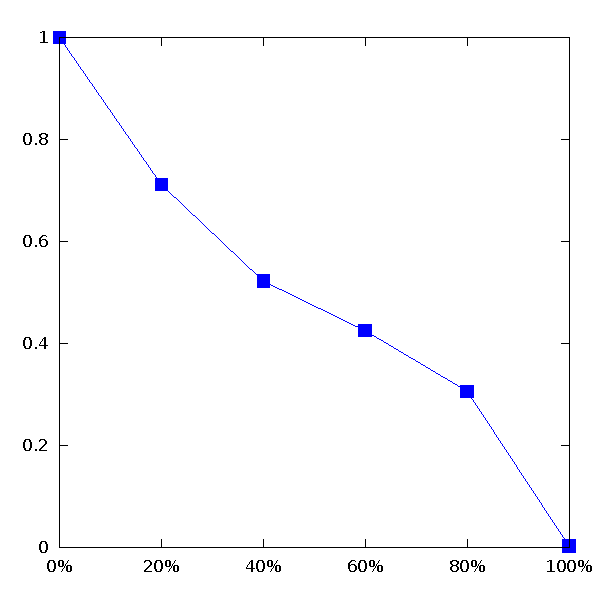
\includegraphics[height=2cm]{allcat_AoD.pdf}
\caption{AoD}
\end{subfigure} 
\begin{subfigure}[b]{2.5cm}
\centering
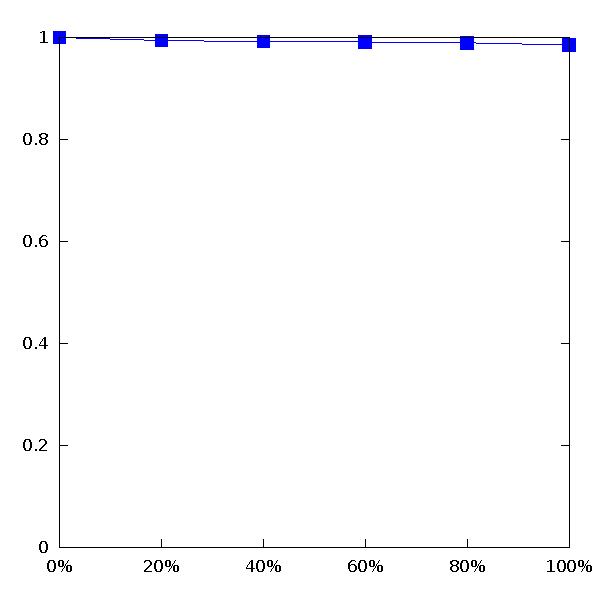
\includegraphics[height=2cm]{allcat_VB-0_5.pdf}
\caption{VB-0.5}
\end{subfigure} 
\begin{subfigure}[b]{2.5cm}
\centering
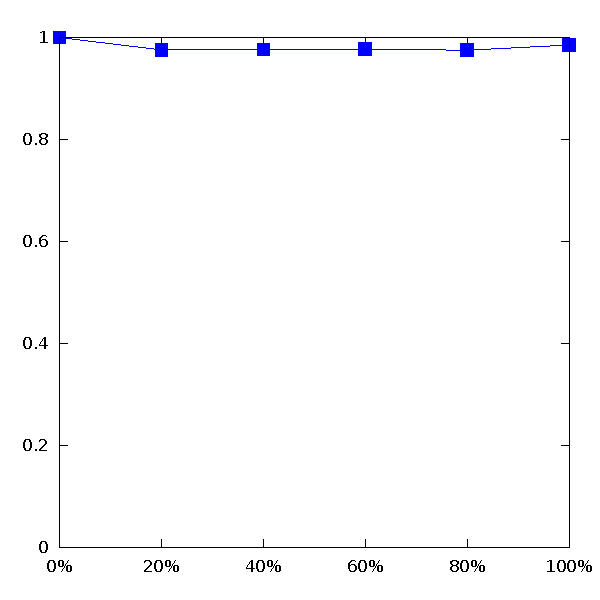
\includegraphics[height=2cm]{allcat_H3D.pdf}
\caption{H3D}
\end{subfigure} 
\begin{subfigure}[b]{2.5cm}
\centering
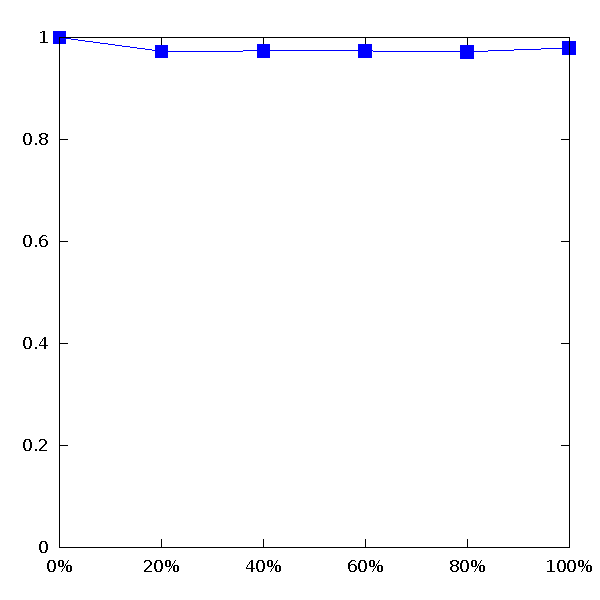
\includegraphics[height=2cm]{allcat_E-3D.pdf}
\caption{E-3D}
\end{subfigure} 
\begin{subfigure}[b]{2.5cm}
\centering
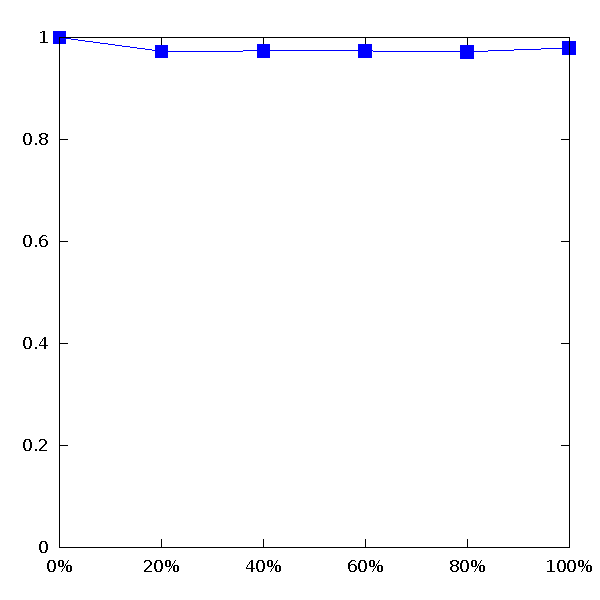
\includegraphics[height=2cm]{allcat_GGeo-3D-2.pdf}
\caption{GGeo-3D-2}
\end{subfigure} 
\begin{subfigure}[b]{2.5cm}
\centering
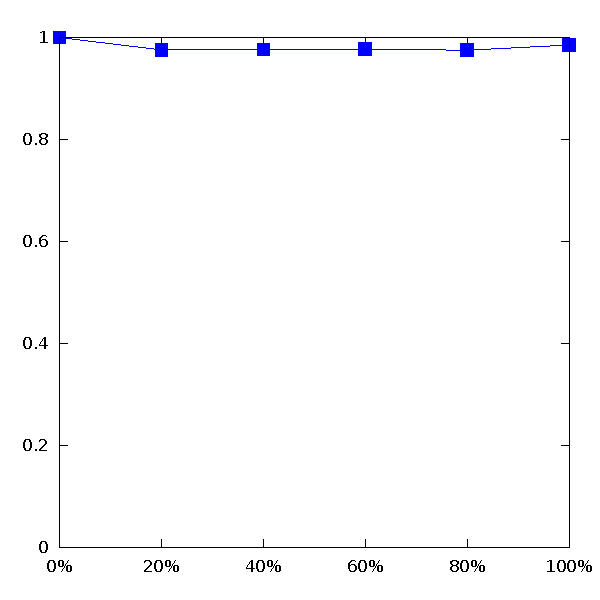
\includegraphics[height=2cm]{allcat_GGeo-3D-1.pdf}
\caption{GGeo-3D-1}
\end{subfigure} 
\begin{subfigure}[b]{2.5cm}
\centering
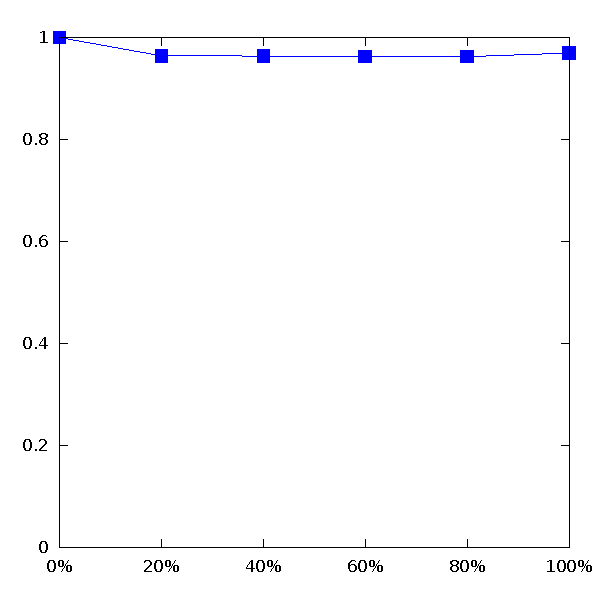
\includegraphics[height=2cm]{allcat_GGeo-3D-4.pdf}
\caption{GGeo-3D-4}
\end{subfigure} 
\begin{subfigure}[b]{2.5cm}
\centering
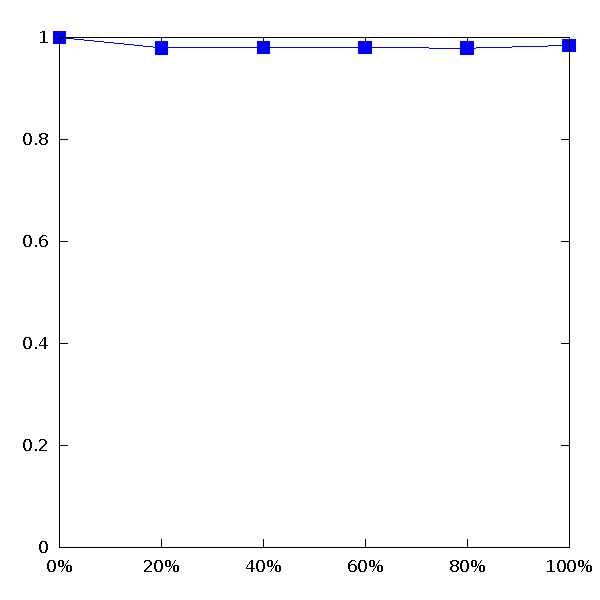
\includegraphics[height=2cm]{allcat_X17-2.pdf}
\caption{X17-2}
\end{subfigure} 
\begin{subfigure}[b]{2.5cm}
\centering
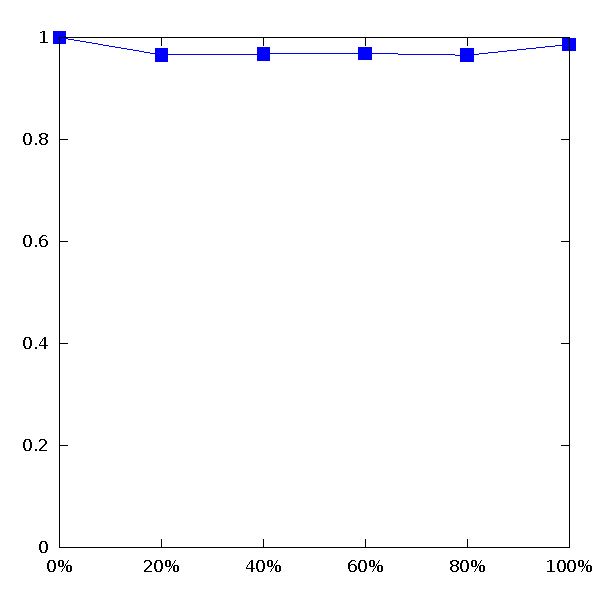
\includegraphics[height=2cm]{allcat_X17-0_5.pdf}
\caption{X17-0.5}
\end{subfigure} 
\begin{subfigure}[b]{2.5cm}
\centering
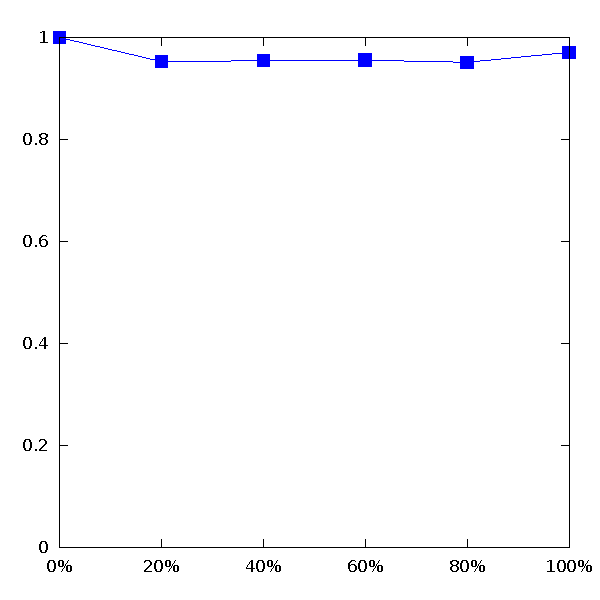
\includegraphics[height=2cm]{allcat_X19.pdf}
\caption{X19}
\end{subfigure} 
\begin{subfigure}[b]{2.5cm}
\centering
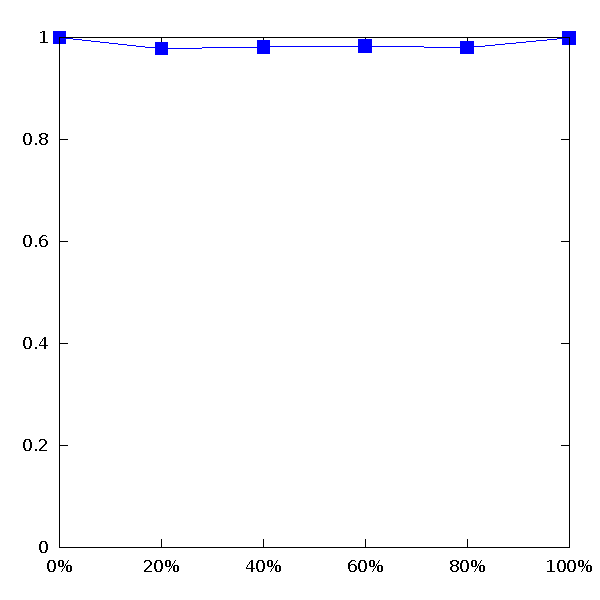
\includegraphics[height=2cm]{allcat_X21.pdf}
\caption{X21}
\end{subfigure} 
\begin{subfigure}[b]{2.5cm}
\centering
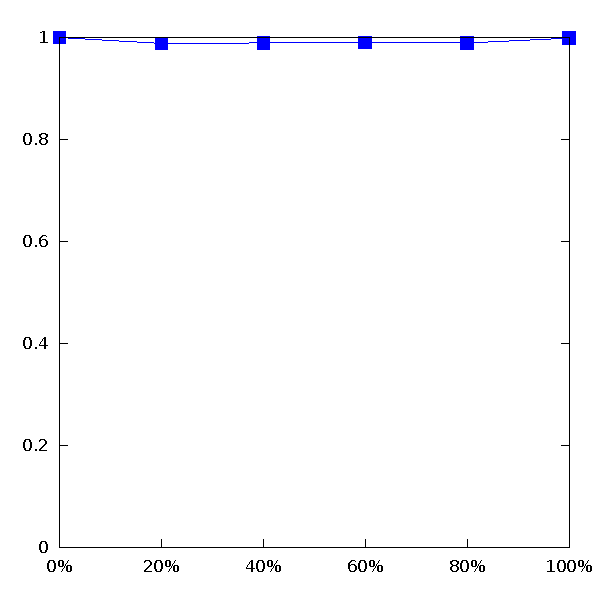
\includegraphics[height=2cm]{allcat_CC.pdf}
\caption{CC}
\end{subfigure} 
\begin{subfigure}[b]{2.5cm}
\centering
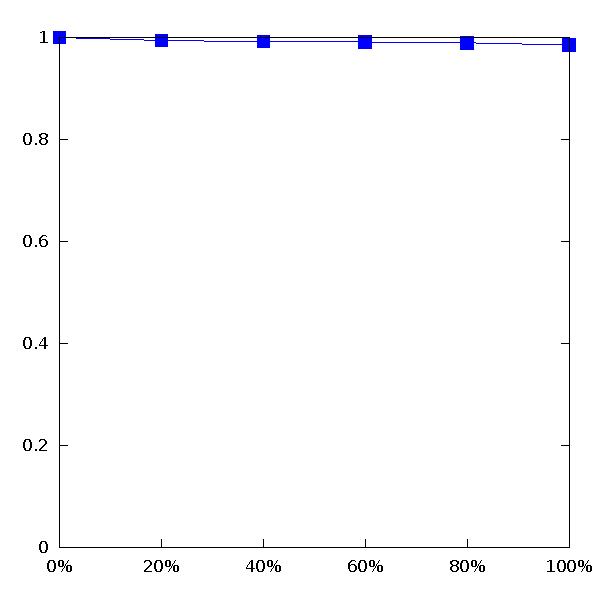
\includegraphics[height=2cm]{allcat_Ch.pdf}
\caption{Ch}
\end{subfigure} 
\begin{subfigure}[b]{2.5cm}
\centering
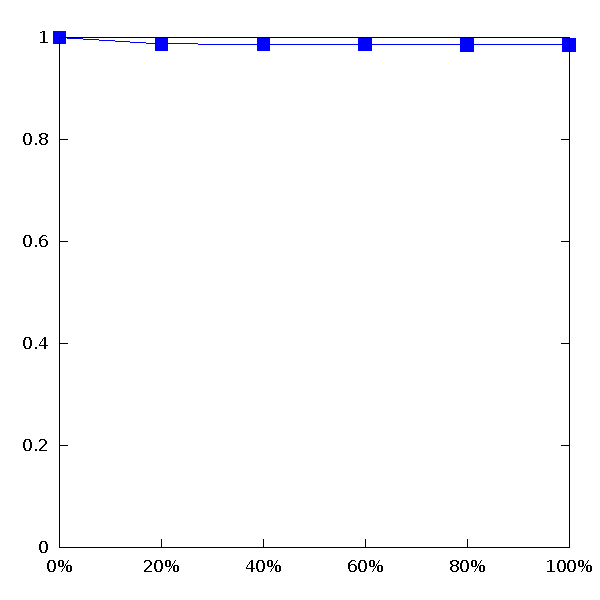
\includegraphics[height=2cm]{allcat_HK.pdf}
\caption{HK}
\end{subfigure} 
\begin{subfigure}[b]{2.5cm}
\centering
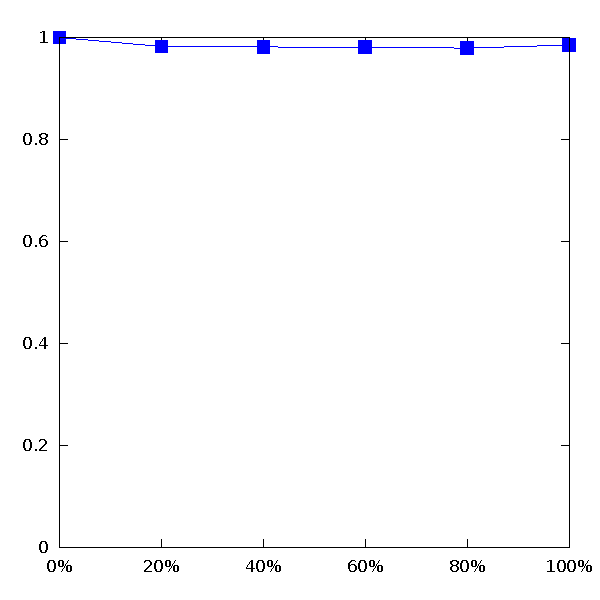
\includegraphics[height=2cm]{allcat_HY15.pdf}
\caption{HY15}
\end{subfigure} 
\begin{subfigure}[b]{2.5cm}
\centering
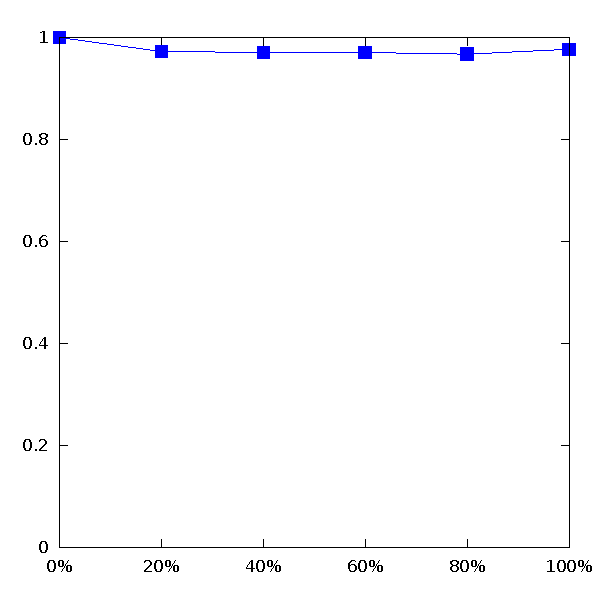
\includegraphics[height=2cm]{allcat_HY16.pdf}
\caption{HY16}
\end{subfigure} 
\begin{subfigure}[b]{2.5cm}
\centering
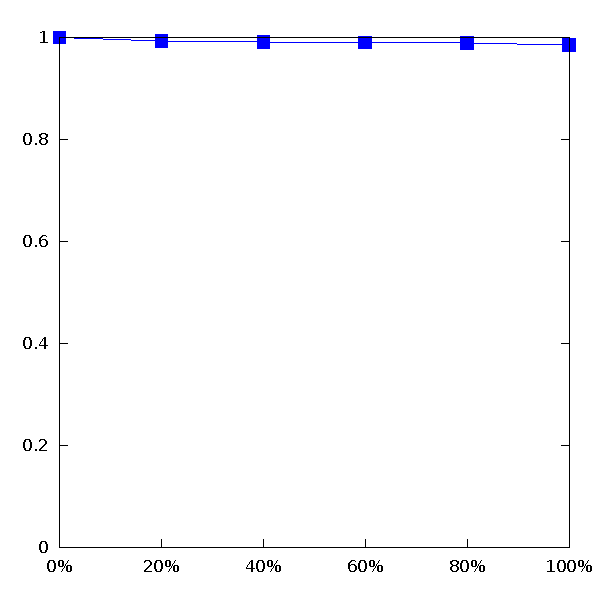
\includegraphics[height=2cm]{allcat_BA-1-2.pdf}
\caption{BA-1-2}
\end{subfigure} 
\begin{subfigure}[b]{2.5cm}
\centering
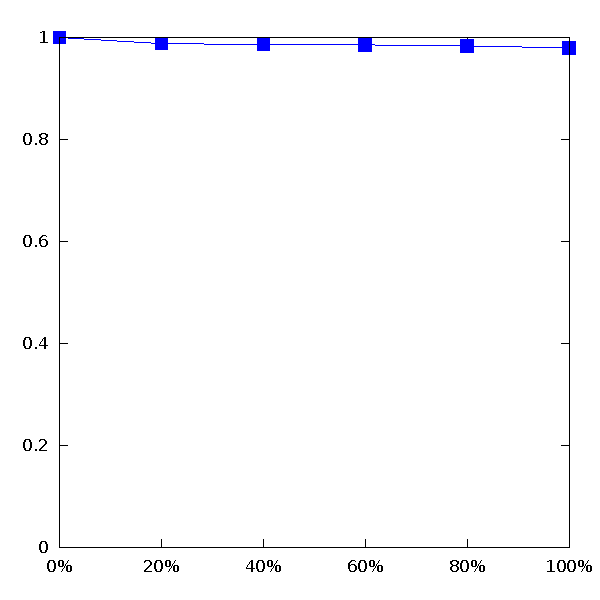
\includegraphics[height=2cm]{allcat_BA-2-4.pdf}
\caption{BA-2-4}
\end{subfigure} 
\begin{subfigure}[b]{2.5cm}
\centering
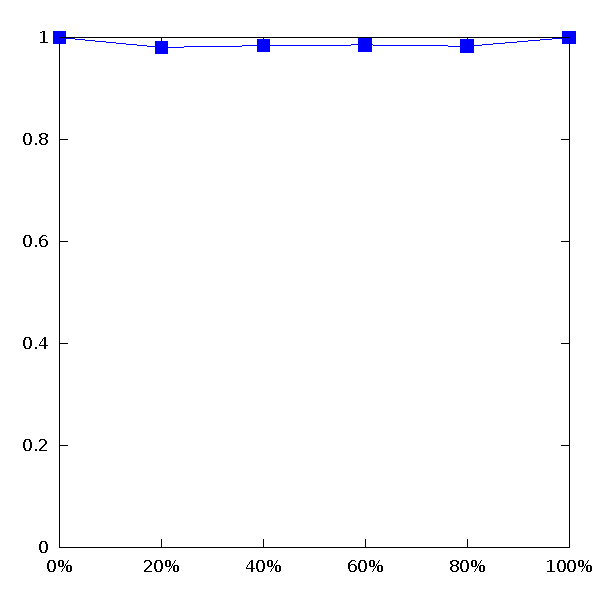
\includegraphics[height=2cm]{allcat_N26.pdf}
\caption{N26}
\end{subfigure} 
\begin{subfigure}[b]{2.5cm}
\centering
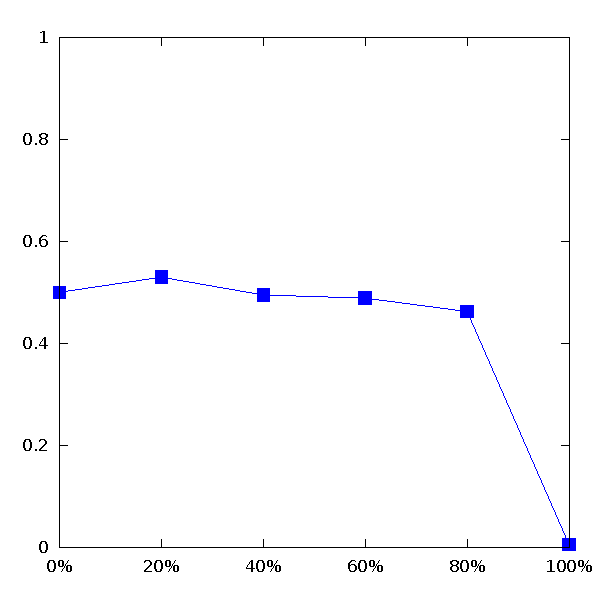
\includegraphics[height=2cm]{allcat_XY19.pdf}
\caption{XY19}
\end{subfigure} 
\caption{Averages of the similarity levels per scenario versus the percentage of opposites included in each scenario (Part 1).}
}\end{figure}
\begin{figure}[ht]{\ContinuedFloat\centering
\begin{subfigure}[b]{2.5cm}
\centering
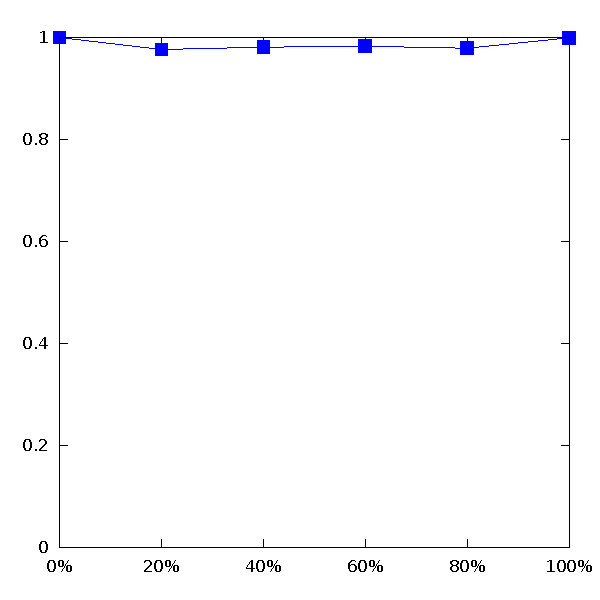
\includegraphics[height=2cm]{allcat_COS.pdf}
\caption{COS}
\end{subfigure} 
\begin{subfigure}[b]{2.5cm}
\centering
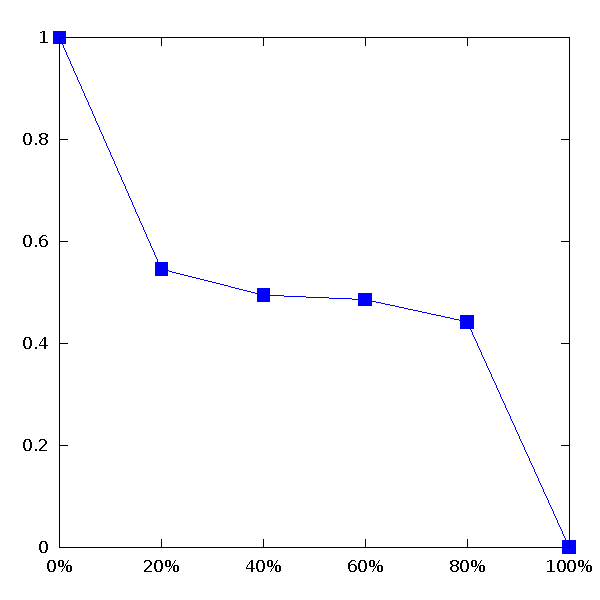
\includegraphics[height=2cm]{allcat_SK1-2D.pdf}
\caption{SK1-2D}
\end{subfigure} 
\begin{subfigure}[b]{2.5cm}
\centering
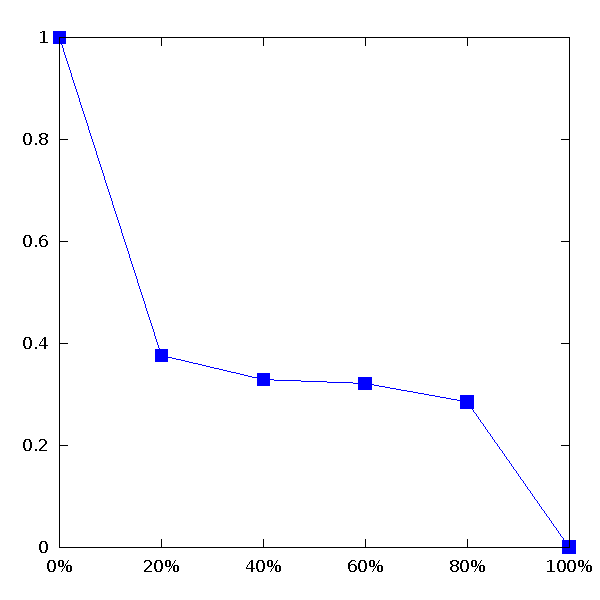
\includegraphics[height=2cm]{allcat_SK2-2D.pdf}
\caption{SK2-2D}
\end{subfigure} 
\begin{subfigure}[b]{2.5cm}
\centering
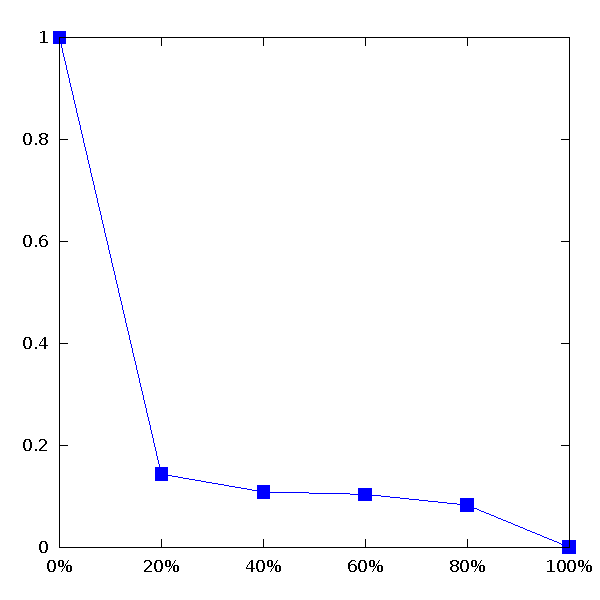
\includegraphics[height=2cm]{allcat_SK3-2D.pdf}
\caption{SK3-2D}
\end{subfigure} 
\begin{subfigure}[b]{2.5cm}
\centering
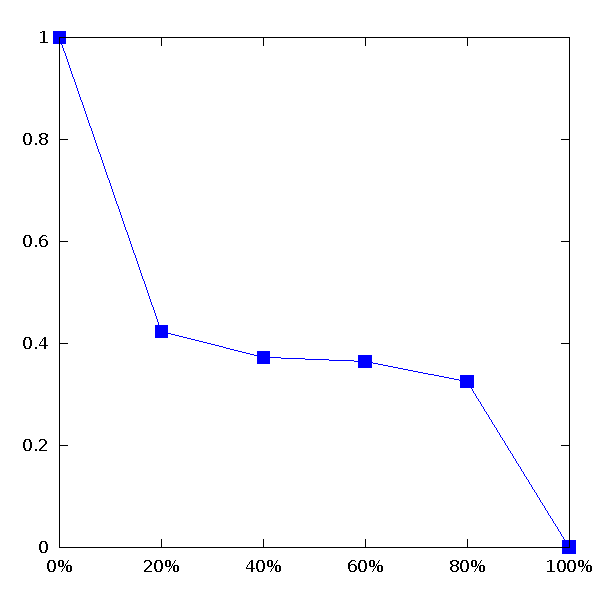
\includegraphics[height=2cm]{allcat_SK4-2D.pdf}
\caption{SK4-2D}
\end{subfigure} 
\begin{subfigure}[b]{2.5cm}
\centering
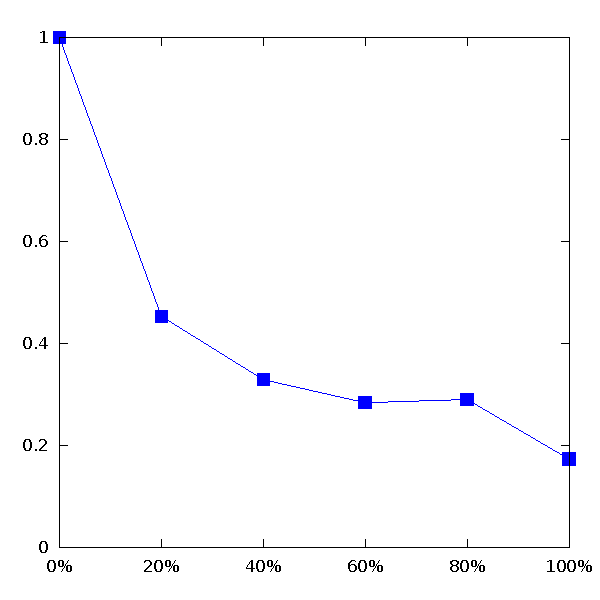
\includegraphics[height=2cm]{allcat_XVB-0-0_05.pdf}
\caption{XVB-0-0.05}
\end{subfigure} 
\begin{subfigure}[b]{2.5cm}
\centering
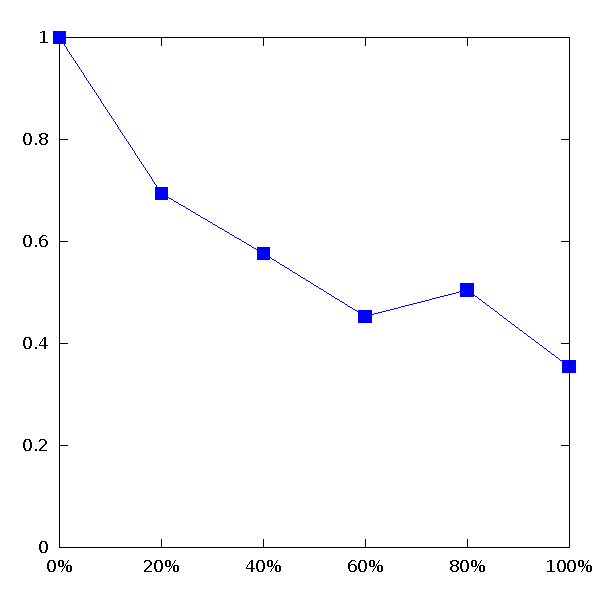
\includegraphics[height=2cm]{allcat_XVB-0-0_1.pdf}
\caption{XVB-0-0.1}
\end{subfigure} 
\begin{subfigure}[b]{2.5cm}
\centering
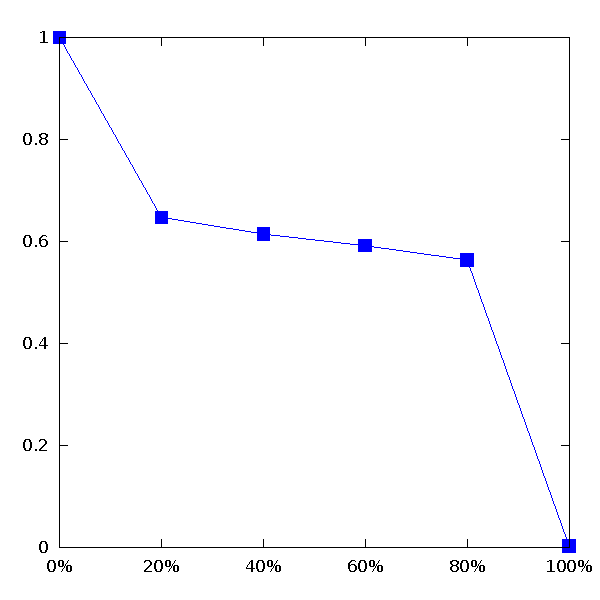
\includegraphics[height=2cm]{allcat_XVBr-1-10.pdf}
\caption{XVBr-1-10}
\end{subfigure} 
\begin{subfigure}[b]{2.5cm}
\centering
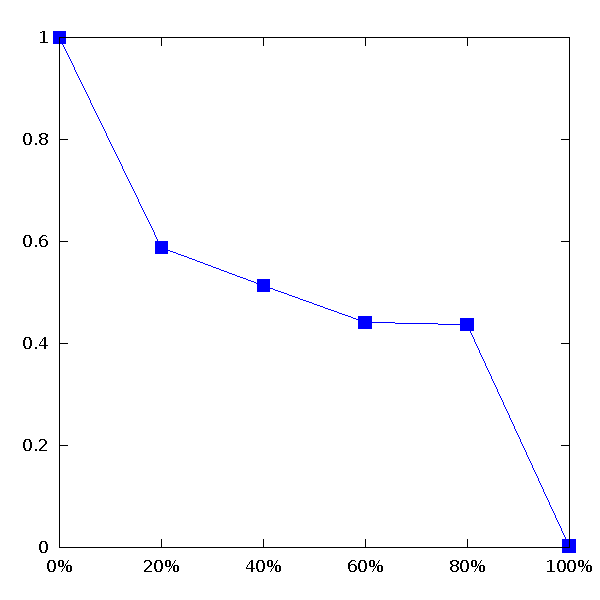
\includegraphics[height=2cm]{allcat_XVBr-0_5-10.pdf}
\caption{XVBr-0.5-10}
\end{subfigure} 
\begin{subfigure}[b]{2.5cm}
\centering
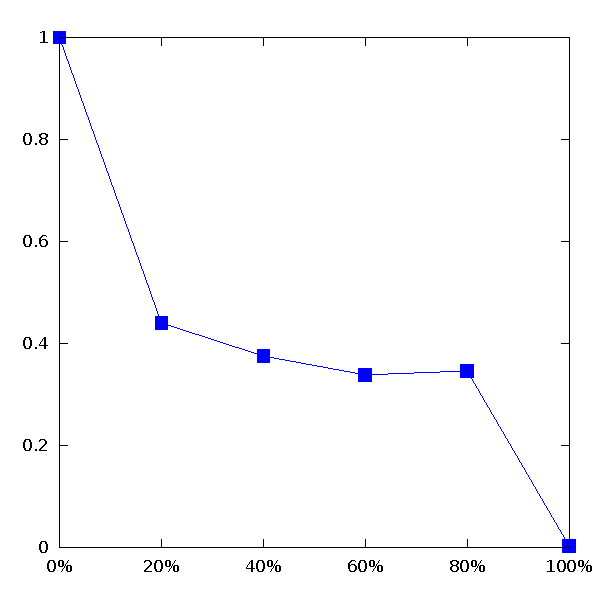
\includegraphics[height=2cm]{allcat_XVBr-0-10.pdf}
\caption{XVBr-0-10}
\end{subfigure} 
\begin{subfigure}[b]{2.5cm}
\centering
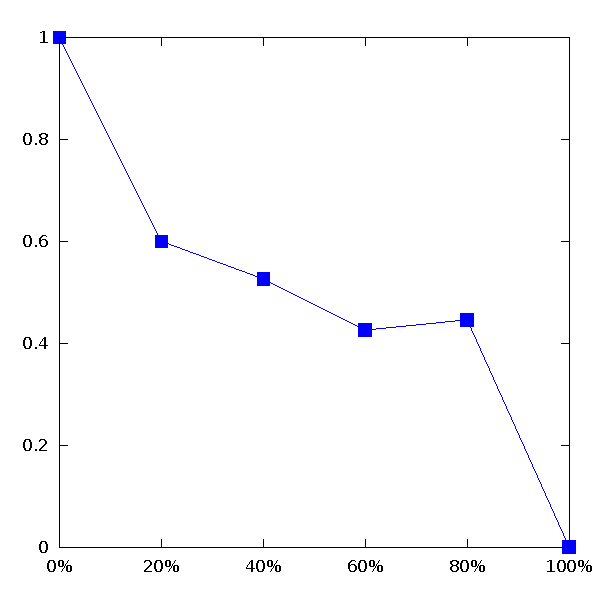
\includegraphics[height=2cm]{allcat_XVBr-1-5.pdf}
\caption{XVBr-1-5}
\end{subfigure} 
\begin{subfigure}[b]{2.5cm}
\centering
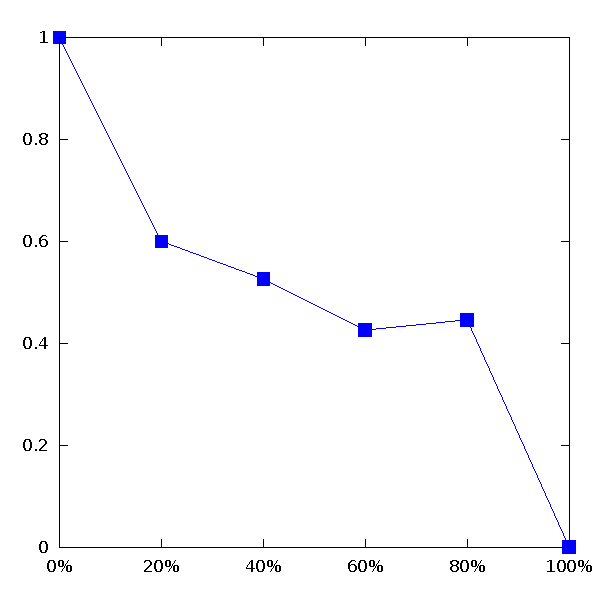
\includegraphics[height=2cm]{allcat_XVBr-0_5-5.pdf}
\caption{XVBr-0.5-5}
\end{subfigure} 
\begin{subfigure}[b]{2.5cm}
\centering
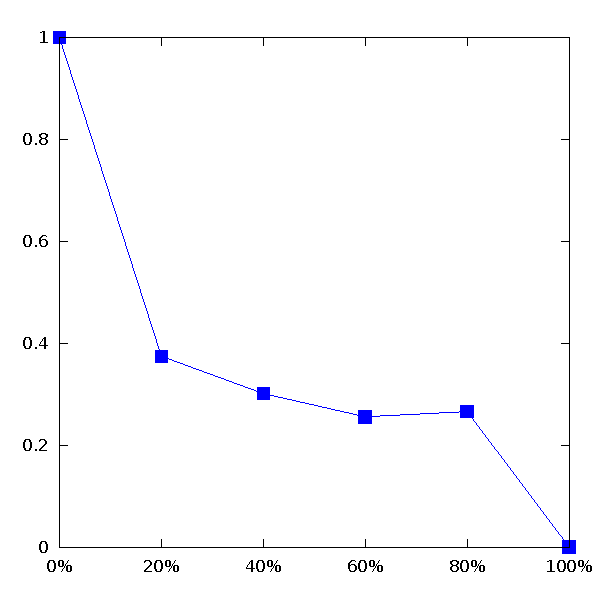
\includegraphics[height=2cm]{allcat_XVBr-0-5.pdf}
\caption{XVBr-0-5}
\end{subfigure} 
\begin{subfigure}[b]{2.5cm}
\centering
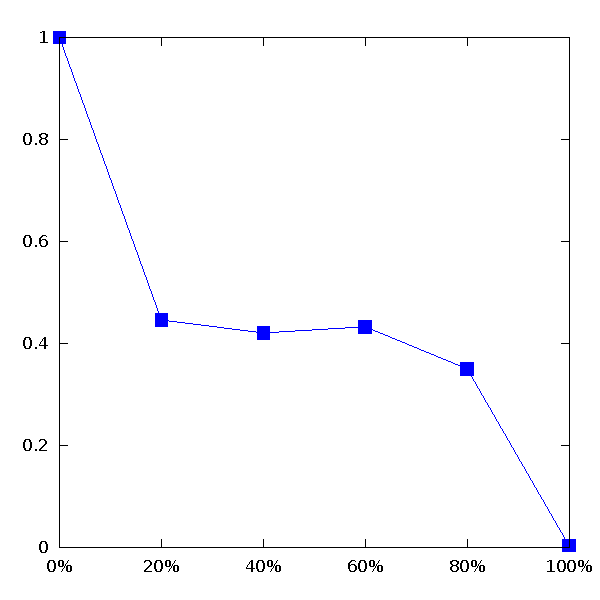
\includegraphics[height=2cm]{allcat_XVBr-1.pdf}
\caption{XVBr-1}
\end{subfigure} 
\begin{subfigure}[b]{2.5cm}
\centering
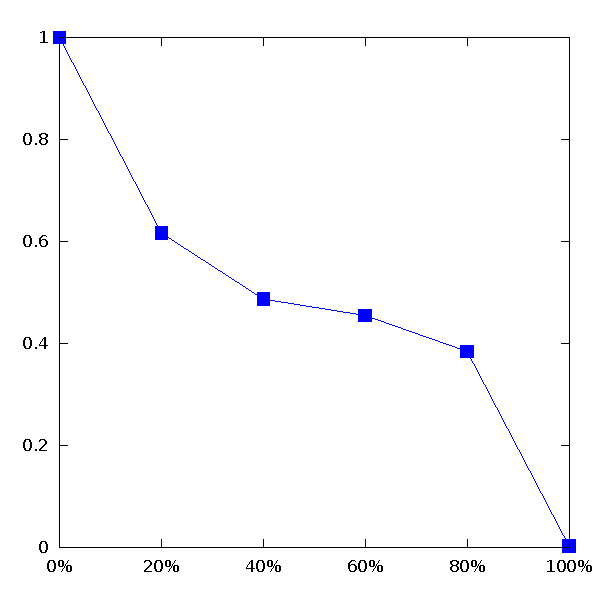
\includegraphics[height=2cm]{allcat_XVBr-0_5.pdf}
\caption{XVBr-0.5}
\end{subfigure} 
\begin{subfigure}[b]{2.5cm}
\centering
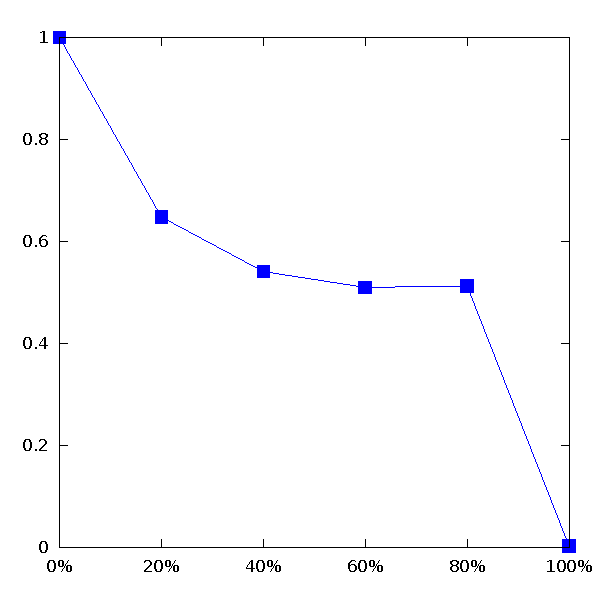
\includegraphics[height=2cm]{allcat_XVBr-0.pdf}
\caption{XVBr-0}
\end{subfigure} 
\caption{Averages of the similarity levels per scenario versus the percentage of opposites included in each scenario (Part 2).}
}\end{figure}
\pagebreak
\subsection{Linear models}
\begin{figure}[ht]{\centering
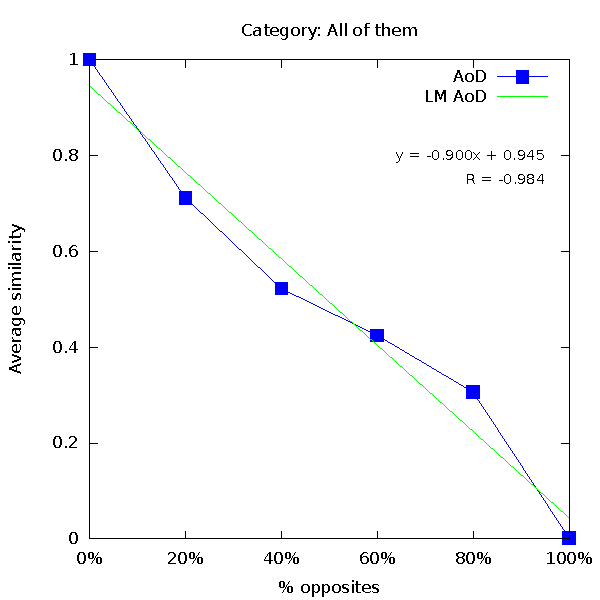
\includegraphics[height=5cm]{allcat_AoD_LM.pdf}
\caption{AoD - Linear model}
}\end{figure}
\begin{figure}[ht]{\centering
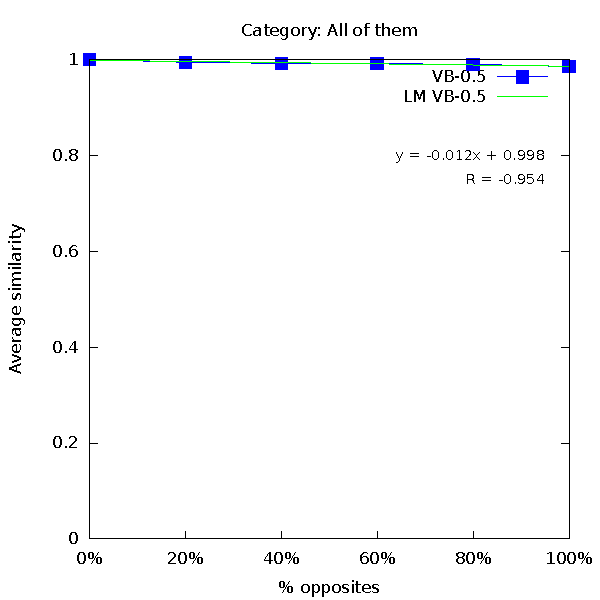
\includegraphics[height=5cm]{allcat_VB-0_5_LM.pdf}
\caption{VB-0.5 - Linear model}
}\end{figure}
\begin{figure}[ht]{\centering
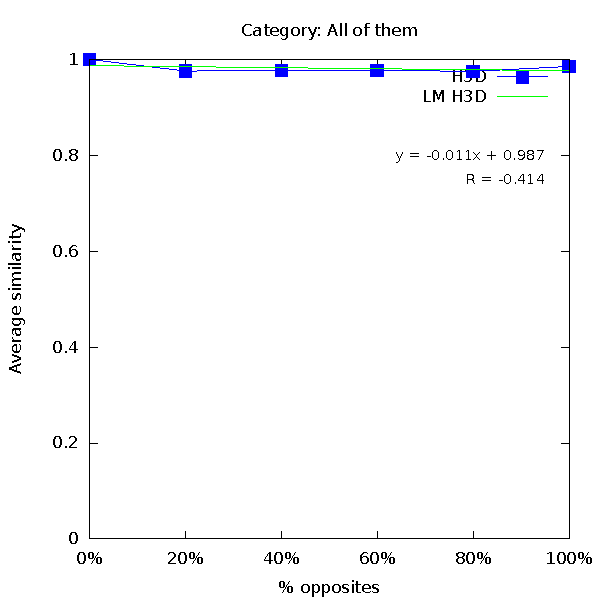
\includegraphics[height=5cm]{allcat_H3D_LM.pdf}
\caption{H3D - Linear model}
}\end{figure}
\begin{figure}[ht]{\centering
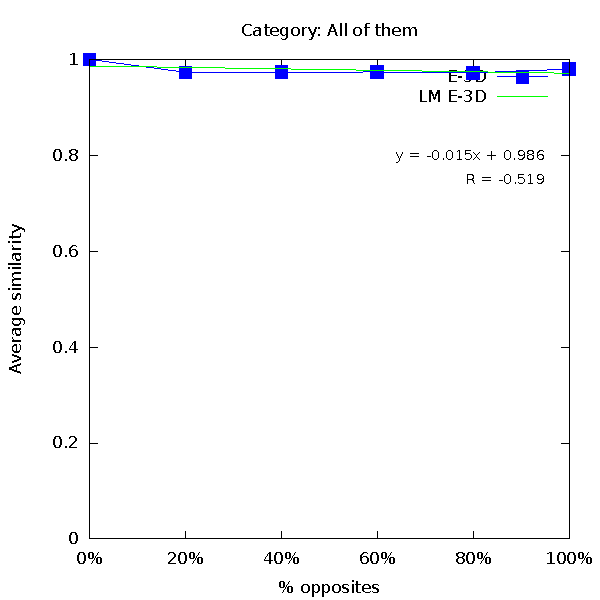
\includegraphics[height=5cm]{allcat_E-3D_LM.pdf}
\caption{E-3D - Linear model}
}\end{figure}
\begin{figure}[ht]{\centering
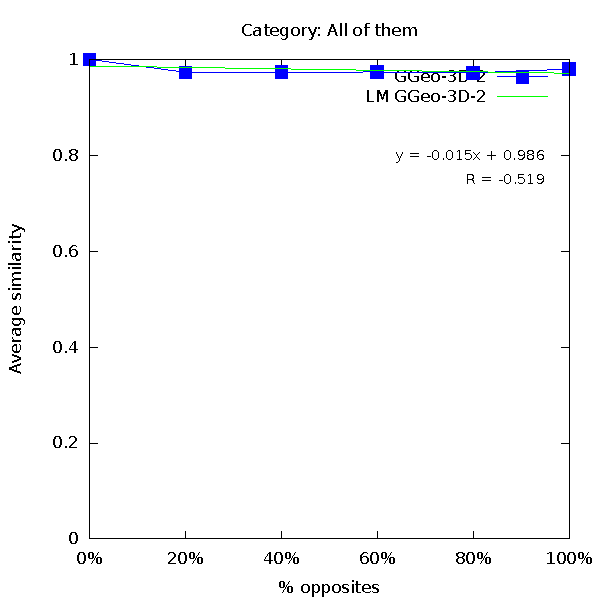
\includegraphics[height=5cm]{allcat_GGeo-3D-2_LM.pdf}
\caption{GGeo-3D-2 - Linear model}
}\end{figure}
\begin{figure}[ht]{\centering
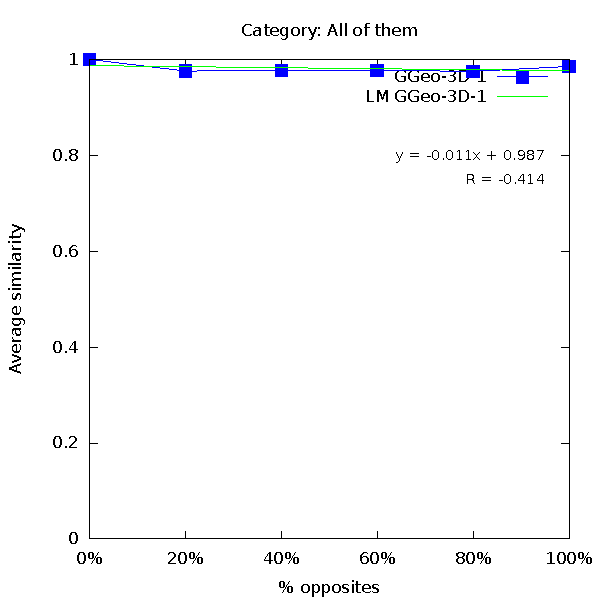
\includegraphics[height=5cm]{allcat_GGeo-3D-1_LM.pdf}
\caption{GGeo-3D-1 - Linear model}
}\end{figure}
\begin{figure}[ht]{\centering
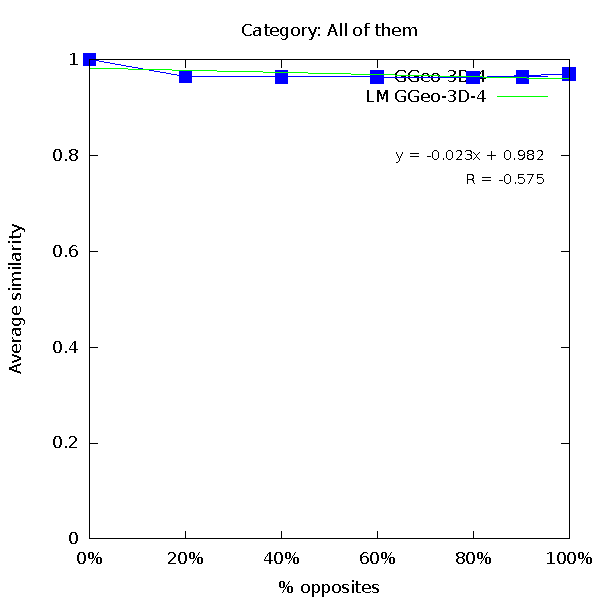
\includegraphics[height=5cm]{allcat_GGeo-3D-4_LM.pdf}
\caption{GGeo-3D-4 - Linear model}
}\end{figure}
\begin{figure}[ht]{\centering
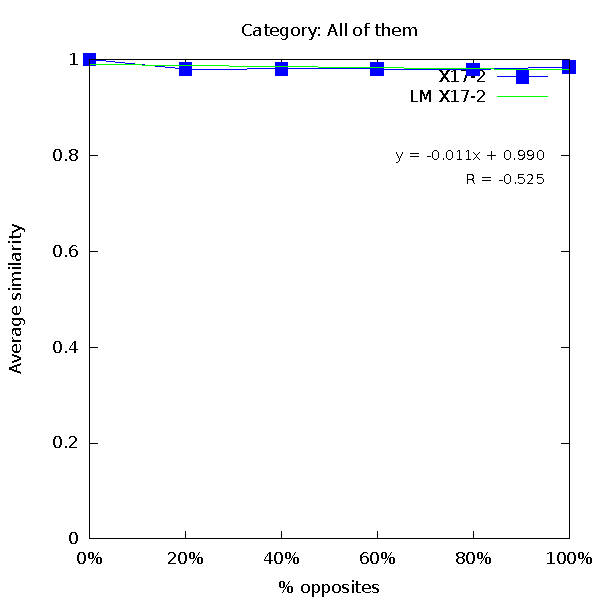
\includegraphics[height=5cm]{allcat_X17-2_LM.pdf}
\caption{X17-2 - Linear model}
}\end{figure}
\begin{figure}[ht]{\centering
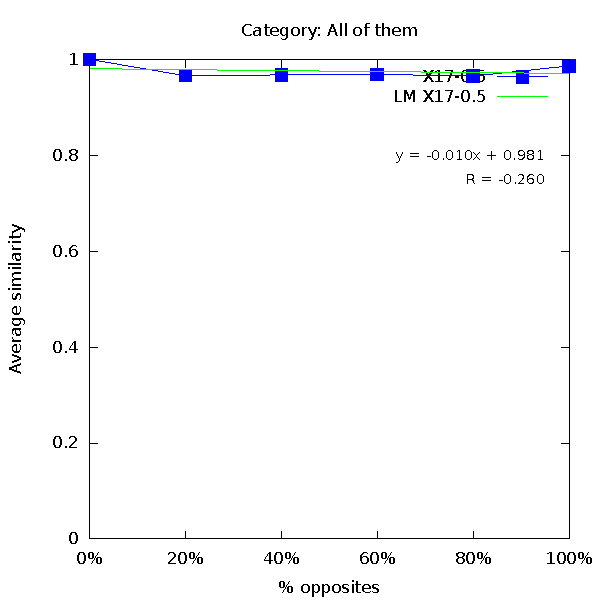
\includegraphics[height=5cm]{allcat_X17-0_5_LM.pdf}
\caption{X17-0.5 - Linear model}
}\end{figure}
\begin{figure}[ht]{\centering
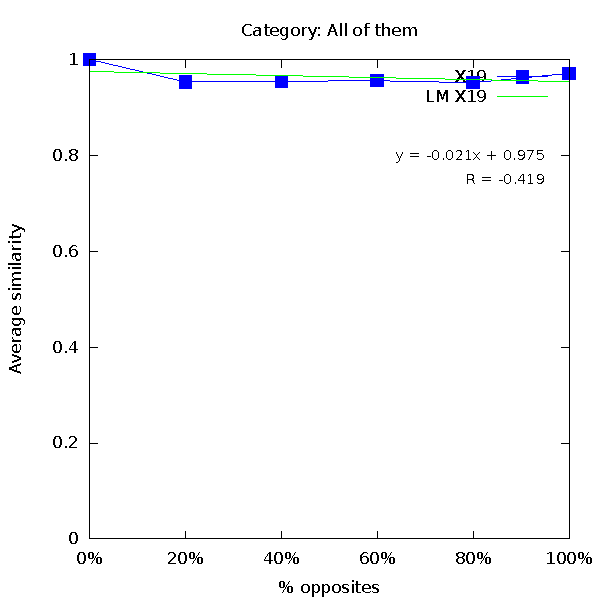
\includegraphics[height=5cm]{allcat_X19_LM.pdf}
\caption{X19 - Linear model}
}\end{figure}
\begin{figure}[ht]{\centering
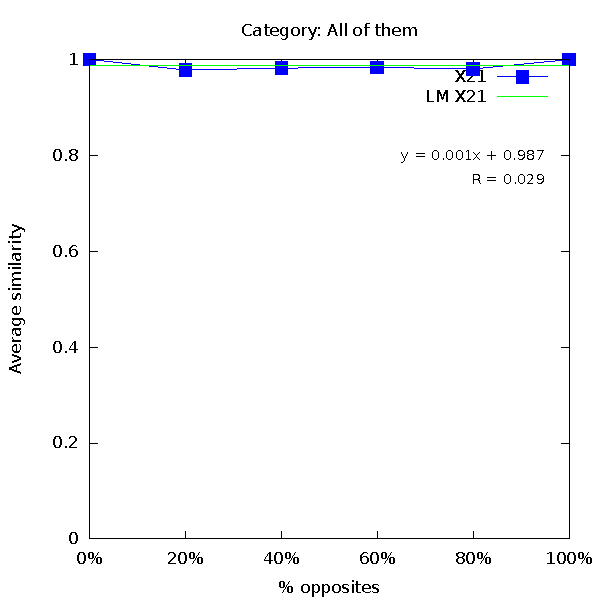
\includegraphics[height=5cm]{allcat_X21_LM.pdf}
\caption{X21 - Linear model}
}\end{figure}
\begin{figure}[ht]{\centering
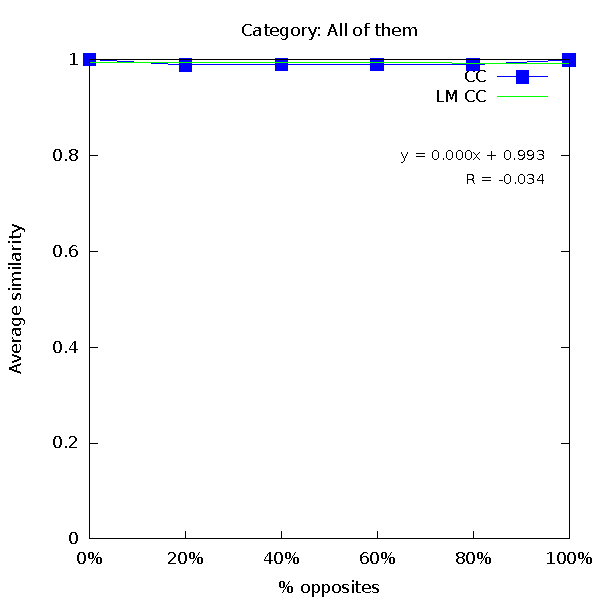
\includegraphics[height=5cm]{allcat_CC_LM.pdf}
\caption{CC - Linear model}
}\end{figure}
\begin{figure}[ht]{\centering
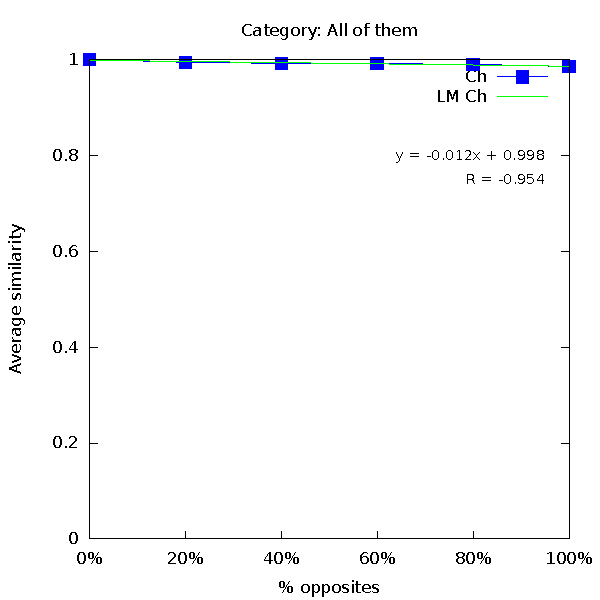
\includegraphics[height=5cm]{allcat_Ch_LM.pdf}
\caption{Ch - Linear model}
}\end{figure}
\begin{figure}[ht]{\centering
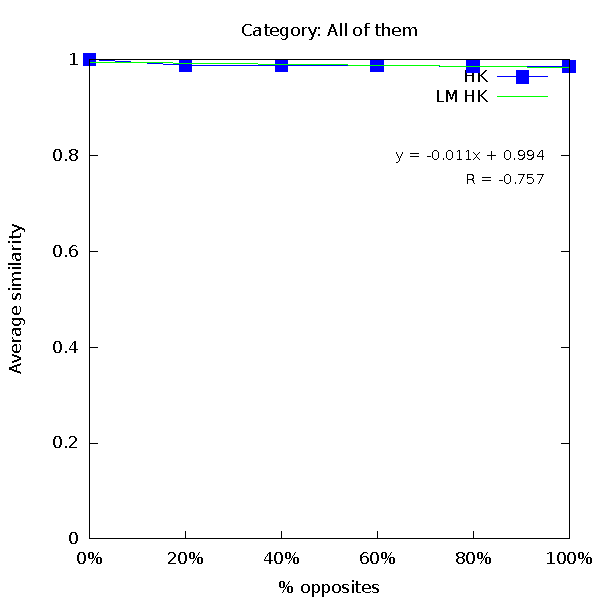
\includegraphics[height=5cm]{allcat_HK_LM.pdf}
\caption{HK - Linear model}
}\end{figure}
\begin{figure}[ht]{\centering
\includegraphics[height=5cm]{allcat_HY15_LM.pdf}
\caption{HY15 - Linear model}
}\end{figure}
\begin{figure}[ht]{\centering
\includegraphics[height=5cm]{allcat_HY16_LM.pdf}
\caption{HY16 - Linear model}
}\end{figure}
\begin{figure}[ht]{\centering
\includegraphics[height=5cm]{allcat_BA-1-2_LM.pdf}
\caption{BA-1-2 - Linear model}
}\end{figure}
\begin{figure}[ht]{\centering
\includegraphics[height=5cm]{allcat_BA-2-4_LM.pdf}
\caption{BA-2-4 - Linear model}
}\end{figure}
\begin{figure}[ht]{\centering
\includegraphics[height=5cm]{allcat_N26_LM.pdf}
\caption{N26 - Linear model}
}\end{figure}
\begin{figure}[ht]{\centering
\includegraphics[height=5cm]{allcat_XY19_LM.pdf}
\caption{XY19 - Linear model}
}\end{figure}
\begin{figure}[ht]{\centering
\includegraphics[height=5cm]{allcat_COS_LM.pdf}
\caption{COS - Linear model}
}\end{figure}
\begin{figure}[ht]{\centering
\includegraphics[height=5cm]{allcat_SK1-2D_LM.pdf}
\caption{SK1-2D - Linear model}
}\end{figure}
\begin{figure}[ht]{\centering
\includegraphics[height=5cm]{allcat_SK2-2D_LM.pdf}
\caption{SK2-2D - Linear model}
}\end{figure}
\begin{figure}[ht]{\centering
\includegraphics[height=5cm]{allcat_SK3-2D_LM.pdf}
\caption{SK3-2D - Linear model}
}\end{figure}
\begin{figure}[ht]{\centering
\includegraphics[height=5cm]{allcat_SK4-2D_LM.pdf}
\caption{SK4-2D - Linear model}
}\end{figure}
\begin{figure}[ht]{\centering
\includegraphics[height=5cm]{allcat_XVB-0-0_05_LM.pdf}
\caption{XVB-0-0.05 - Linear model}
}\end{figure}
\begin{figure}[ht]{\centering
\includegraphics[height=5cm]{allcat_XVB-0-0_1_LM.pdf}
\caption{XVB-0-0.1 - Linear model}
}\end{figure}
\begin{figure}[ht]{\centering
\includegraphics[height=5cm]{allcat_XVBr-1-10_LM.pdf}
\caption{XVBr-1-10 - Linear model}
}\end{figure}
\begin{figure}[ht]{\centering
\includegraphics[height=5cm]{allcat_XVBr-0_5-10_LM.pdf}
\caption{XVBr-0.5-10 - Linear model}
}\end{figure}
\begin{figure}[ht]{\centering
\includegraphics[height=5cm]{allcat_XVBr-0-10_LM.pdf}
\caption{XVBr-0-10 - Linear model}
}\end{figure}
\begin{figure}[ht]{\centering
\includegraphics[height=5cm]{allcat_XVBr-1-5_LM.pdf}
\caption{XVBr-1-5 - Linear model}
}\end{figure}
\begin{figure}[ht]{\centering
\includegraphics[height=5cm]{allcat_XVBr-0_5-5_LM.pdf}
\caption{XVBr-0.5-5 - Linear model}
}\end{figure}
\begin{figure}[ht]{\centering
\includegraphics[height=5cm]{allcat_XVBr-0-5_LM.pdf}
\caption{XVBr-0-5 - Linear model}
}\end{figure}
\begin{figure}[ht]{\centering
\includegraphics[height=5cm]{allcat_XVBr-1_LM.pdf}
\caption{XVBr-1 - Linear model}
}\end{figure}
\begin{figure}[ht]{\centering
\includegraphics[height=5cm]{allcat_XVBr-0_5_LM.pdf}
\caption{XVBr-0.5 - Linear model}
}\end{figure}
\begin{figure}[ht]{\centering
\includegraphics[height=5cm]{allcat_XVBr-0_LM.pdf}
\caption{XVBr-0 - Linear model}
}\end{figure}
\begin{thebibliography}{00}
\bibitem{Loor2017} Loor, M., De Tr{\'e}, G.: In a Quest for Suitable Similarity Measures to Compare Experience-Based Evaluations. In: Computational Intelligence: International Joint Conference, IJCCI 2015 Lisbon, Portugal, November 12-14, 2015, Revised Selected Papers pp. 291-314 (2017)
\bibitem{Loor2013} M.~Loor and G.~De~Tr{\'e}, ``{{Vector Based Similarity Measure for Intuitionistic Fuzzy Sets}},'' in \emph{{{Modern Approaches in Fuzzy Sets, Intuitionistic Fuzzy Sets, Generalized Nets and Related Topics : Volume I: Foundations}}}, K.~T. Atanassov, M.~Baczy{\'n}ski, J.~Drewniak, J.~Kacprzyk, M.~Krawczak, E.~Szmidt, M.~Wygralak, and S.~Zadro{\.z}ny, Eds. SRI-PAS, 2014, pp. 105--127.
\bibitem{Szmidt2000} E.~Szmidt and J.~Kacprzyk, ``{Distances between intuitionistic fuzzy sets},'' \emph{Fuzzy Sets and Systems}, vol. 114, no.~3, pp. 505--518, Sep. 2000.
\bibitem{Xu2007} Z.~Xu, ``Some similarity measures of intuitionistic fuzzy sets and their applications to multiple attribute decision making,'' \emph{Fuzzy Optimization and Decision Making}, vol.~6, no.~2, pp. 109--121, 2007.
\bibitem{Chen2016} S.-M. Chen, S.-H. Cheng, and T.-C. Lan, ``A novel similarity measure between intuitionistic fuzzy sets based on the centroid points of transformed fuzzy numbers with applications to pattern recognition,'' \emph{Information Sciences}, vol. 343--344, pp. 15 -- 40, 2016.
\bibitem{Chen1997} S.-M. Chen \emph{et~al.}, ``Similarity measures between vague sets and between elements,'' \emph{IEEE TRANSACTIONS ON SYSTEMS MAN AND CYBERNETICS PART B-CYBERNETICS}, vol.~27, no.~1, pp. 153--158, 1997.
\bibitem{Hong1999} D.~H. Hong and C.~Kim, ``A note on similarity measures between vague sets and between elements,'' \emph{Information Sciences}, vol. 115, no.~1, pp. 83 --
  96, 1999.
\bibitem{Hung2004} W.-L. Hung and M.-S. Yang, ``Similarity measures of intuitionistic fuzzy sets based on Hausdorff distance,'' \emph{Pattern Recognition Letters}, vol.~25, no.~14, pp. 1603 -- 1611, 2004.
\bibitem{Boran2014} F.~E. Boran and D.~Akay, ``A biparametric similarity measure on intuitionistic fuzzy sets with applications to pattern recognition,'' \emph{Information Sciences}, vol. 255, pp. 45 -- 57, 2014.
\bibitem{Nguyen2016} H.~Nguyen, ``A novel similarity/dissimilarity measure for intuitionistic fuzzy sets and its application in pattern recognition,'' \emph{Expert Systems with Applications}, vol.~45, pp. 97 -- 107, 2016.
\bibitem{Xu2009} Z.~Xu and R.~R. Yager, ``Intuitionistic and interval-valued intutionistic fuzzy preference relations and their measures of similarity for the evaluation of agreement within a group,'' \emph{Fuzzy Optimization and Decision Making},  vol.~8, no.~2, pp. 123--139, 2009.
\bibitem{Szmidt2013} ``Geometric similarity measures for the intuitionistic fuzzy sets,'' in \emph{8th conference of the European Society for Fuzzy Logic and Technology  (EUSFLAT-13)}. Atlantis Press, 2013,  pp. 840--847.
\bibitem{Szmidt2004} E.~Szmidt and J.~Kacprzyk, ``A concept of similarity for intuitionistic fuzzy sets and its use in group decision making,'' in \emph{IEEE International Conference on Fuzzy Systems}, 2004, pp. 1129--1134.
\end{thebibliography}
 \end{document}
